\subsection{The \macro{ROOTGRAM}}\label{discrete-root}
The \macro{ROOTGRAM} (\macref{mac:rootgram}) displays observed and fitted frequencies
for a \Dset\ in any of the forms shown in \figref{fig:madfit}.
The input \Dset\ is usually of the form of the output
\texttt{OUT=} \Dset\ produced by the \macro{GOODFIT}.

\begin{Example}[federalist2]{Federalist papers}
We have seen that the negative binomial produces a better fit to the
Federalist Papers data.  The hanging rootogram (\figref{fig:madfit5}),
produced by the statements below, is characteristic of a decent fit.
\begin{listing}
%include catdata(madison);
%goodfit(data=madison, var=count, freq=blocks, dist=negbin, out=fit2);
%rootgram(data=fit2, var=count, obs=blocks, btype=dev);
\end{listing}
%\begin{figure}
%\fig{madfit5.eps}{scale=.7}{madfit5}{Hanging rootogram for the Federalist Papers data, Negative binomial model}
\fig{madfit5}{scale=.7}{Hanging rootogram for the Federalist Papers data, Negative binomial model}
%\end{figure}
\end{Example}


\begin{Example}[saxony1]{Families in Saxony}
Geissler
(cited in \citet{SokalRholf:69}
and \citet{Lindsey:95})
tabulated a huge \Dset\ on sex distributions in families in Saxony
in the 19th century.  Included were $N=6115$ families with $n=12$ children,
which might reasonably be expected to follow a Bin(12,$p$) distribution.
The data are input and fit as shown below.
%% input: /users/faculty/friendly/sasuser/catdata/saxony.sas
%% last modified: 08-Jan-98  9:29
\begin{listing}
title 'Number of males in 6115 families in Saxony';
data saxony;
   do males = 0 to 12;
      input families @;
      output;
      end;
   label males='Number of males'
      families='Number of families';
datalines;
3  24  104  286  670  1033  1343 1112  829  478  181  45  7
;

%goodfit(data=saxony, var=males, freq=families, dist=binomial);

title;
%rootgram(data=fit, var=males, obs=families, exp=exp);
\end{listing}


The fitted distribution, using the estimated proportion of males,
$p = .5192$ is shown in \outref{out:saxony.1};
the goodness of fit tests shown in \outref{out:saxony.2}
indicate that the fit of the Binomial is not good.
The hanging rootogram in \figref{fig:saxony} shows why---%
there is a systematic pattern of deviations from the Binomial,
which produces fitted frequencies too high in the middle and too small
in the tails.
The lack of fit might be ascribed to violations of the assumptions---%
a constant probability of a male birth over a long time span
is a good possibility.
\footnote{\citet[p. 131]{Lindsey:95}
fits a double binomial model with one extra parameter,
and achieves a much better fit, but this too
shows significant lack of fit, not surprising considering the
enormous sample size.}
\begin{Output}
\caption{Fit of the Binomial($12, p$) to the Families in Saxony data: Observed and fitted frequencies}\label{out:saxony.1}
\small
\verbatiminput{ch2/out/saxony.1}
\end{Output}
\begin{Output}
\caption{Fit of the Binomial($12, p$) to the Families in Saxiony data: Goodness of fit tests}\label{out:saxony.2}
\small
\verbatiminput{ch2/out/saxony.2}
\end{Output}

\begin{figure}[htb]
  \centering
  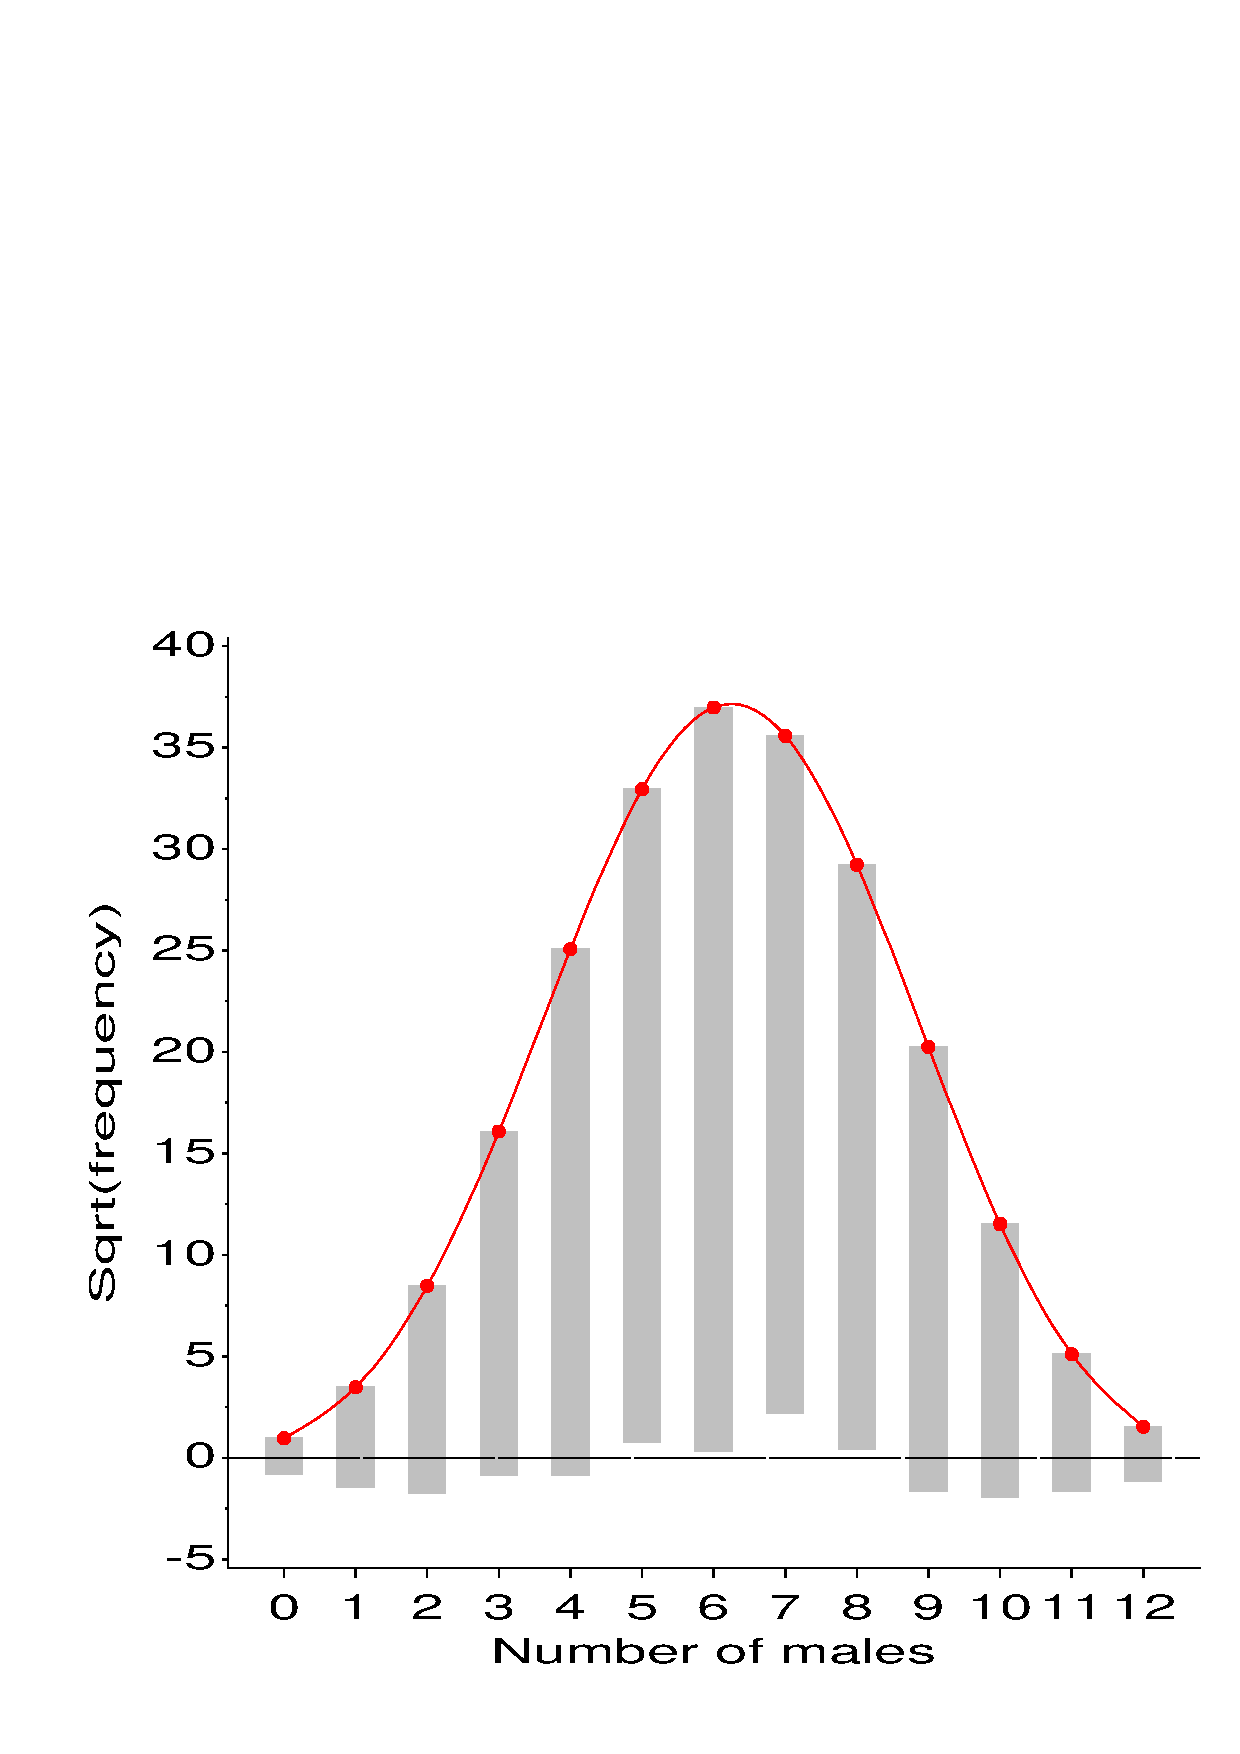
\includegraphics[scale=.5]{saxony}\graphicsfile{ch2/fig/saxony.eps}{}
  \caption[Hanging rootogram for Saxony families, Binomial model]{Hanging rootogram for Saxony families, Binomial($12, p$) model.
The systematic pattern of deviations shows that the Binomial model is not completely adequate for these data.}\label{fig:saxony}
\end{figure}
\end{Example}

